\section{Алгоритм работы программы}

Пусть $\psi(t)$~--- решение сопряженной системы, тогда $\lambda\psi(t)$ также является решением этой системы. В таком случае, не ограничивая общности, можем положить $\|\psi(t_0)\| = 1$. Поэтому для решения поставленной задачи можно организовать перебор $\psi(t_0)$ по единичной окружности и решить сопряженную систему для начального условия $\psi(t_0)$. Затем, применяя условие трансверсальности для левого конца, можем найти значение $x(t_0)$ для перебираемого $\psi(t_0)$:
$$
        \rho(\psi(t_0)\,|\,\X_0) = \langle\psi(t_0),\,x_0\rangle + r\|\psi(t_0)\| = \langle\psi(t_0),\,x(t_0)\rangle
$$
$$
        x^*(t_0) = x_0 + r\psi(t_0). 
$$

Из принципа максимума найдем допустимые управления $u(t)$:
$$
        \langle B^\T(t)\psi(t),\,u(t)\rangle = \rho(B^\T(t)\psi(t)\,|\,\Omega).
$$
Положив $l(t) = B^\T(t)\psi(t)$, получаем, что $u(t)$ есть опорный вектор множества $\Omega$ в направлении $l(t)$.

Условие трансверсальности на правом конце утверждает, что вектор $\psi(t_1)$ и вектор внешней нормали целевого множества в точке $x(t_1)$ сонаправлены. Таким образом, мы можем ввести погрешность выполнения условия трансверсальности на правом конце по соотношением
$$
        \delta = \frac{\langle-\psi(t_1),\,n\rangle}{\|\psi(t_1)\|}.
$$
\begin{figure}[h]
        \noindent
        \centering
        {
                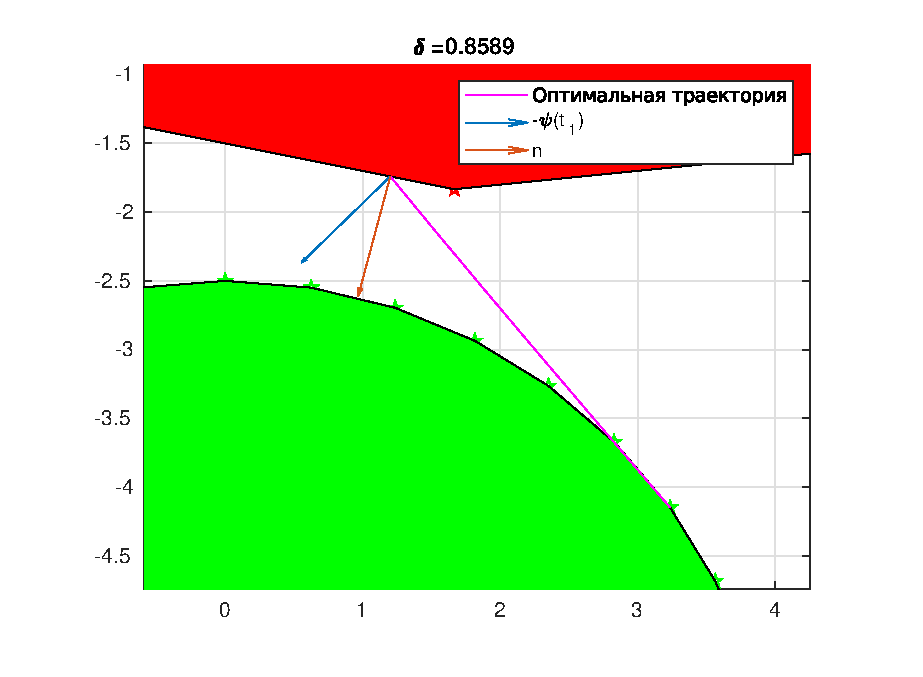
\includegraphics[width=120mm]{algorithm/transvers.eps}
        }
        \caption{Пример посчитанной погрешности условия трансверсальности на правом конце.}
\end{figure}

Исходя из вышеприведенных рассуждений выделим основные этапы численного решения задачи быстродействия \eqref{eq:main_system}:
\begin{enumerate}
        \item Перебор начальных значений $\psi(t_0)$ по единичной окружности.
        \item Численное решение сопряженной задачи Коши для каждого начального условия $\psi(t_0)$ из перебираемых.
        \item Нахождение множества потенциально оптимальных по быстродействию управлений из условия максимума для каждого из перебираемых $\psi(t_0)$.
        \item Нахождение траектории, соответствующей каждому из потенциальных управлений.
        \item Проверка полученных траекторий на попадание в целевое множество $\X_1$.
        \item Отсекаем из множества потенциальных управлений те, соответствующие траектории которых не достигли целевого множества за некоторое задаваемое пользователем время $T_{\max}$.
        \item Выделяем из всех получившихся управлений такое, соответствующая траектория которого достигает целевого множества за кратчайшее время. В случае, если такая траектория единственна, считаем её оптимальной по быстродействию траекторией для задачи \eqref{eq:main_system}.
\end{enumerate}

\subsection{Методы улучшения точности алгоритма}

В рамках задания реализованы следующие методы улучшения точности результата:
\begin{description}
        \item[Глобальный.] Происходит равномерное увеличение количества узлов сетки при переборе начального значения сопряженной переменной $\psi(t_0)$ на всей единичной окружности. Таким образом увеличивается количество построенных траекторий по всех направлениям.
        \begin{figure}[h]
                \hfill
                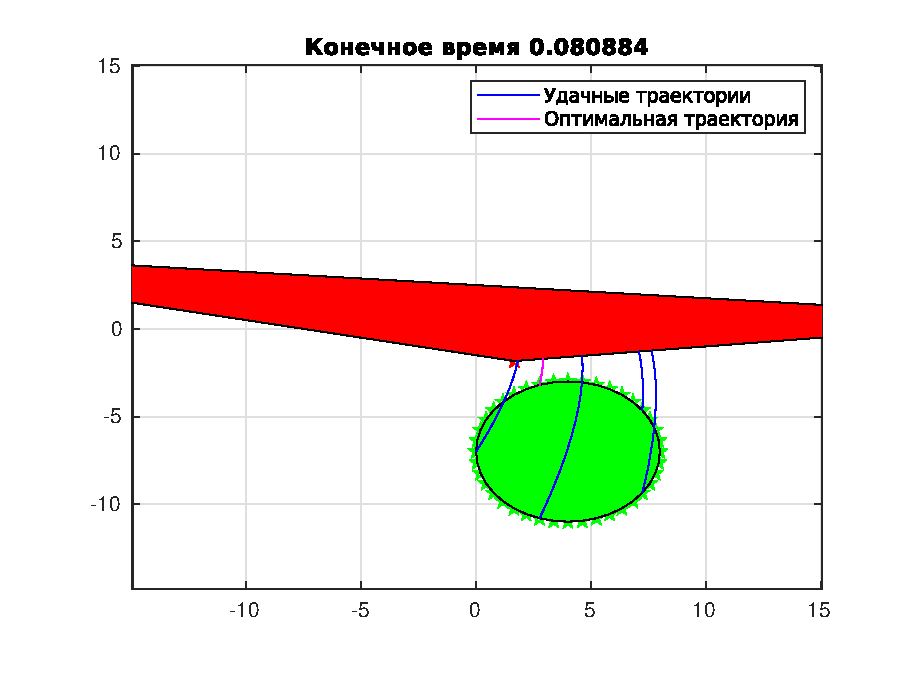
\includegraphics[width=70mm]{algorithm/glb-imp-1.eps}
                \hfill
                \hfill
                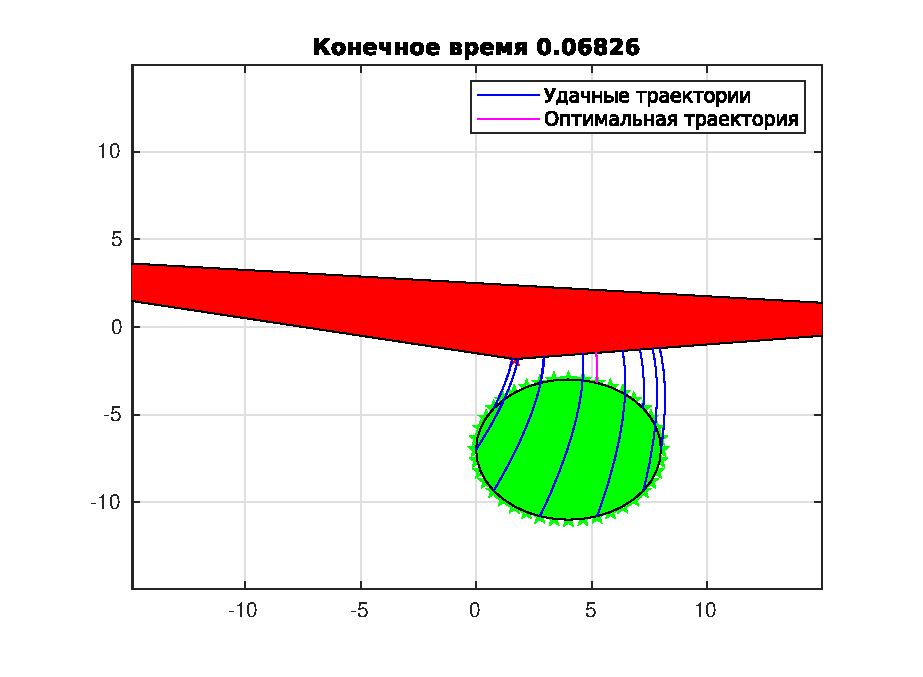
\includegraphics[width=70mm]{algorithm/glb-imp-2.eps}
                \hfill
                \caption{Пример глобального увеличения точности алгоритма.}
        \end{figure}
        \item[Локальный.] Увеличение количества узлов сетки в окрестности некоторой точки. Таким образом, мы получим увеличение числа траекторий в конкретном направлении. Это может быть полезно, когда мы знаем ,,оптимальное‘‘ значение сопряженной переменной $\psi^*(t)$ для предыдущей итерации работы программы. В таком случае полезно рассматривать траектории, выпущенные из некоторой окрестности точки $\psi^*(t_0)$.

        \begin{figure}[h]
                \hfill
                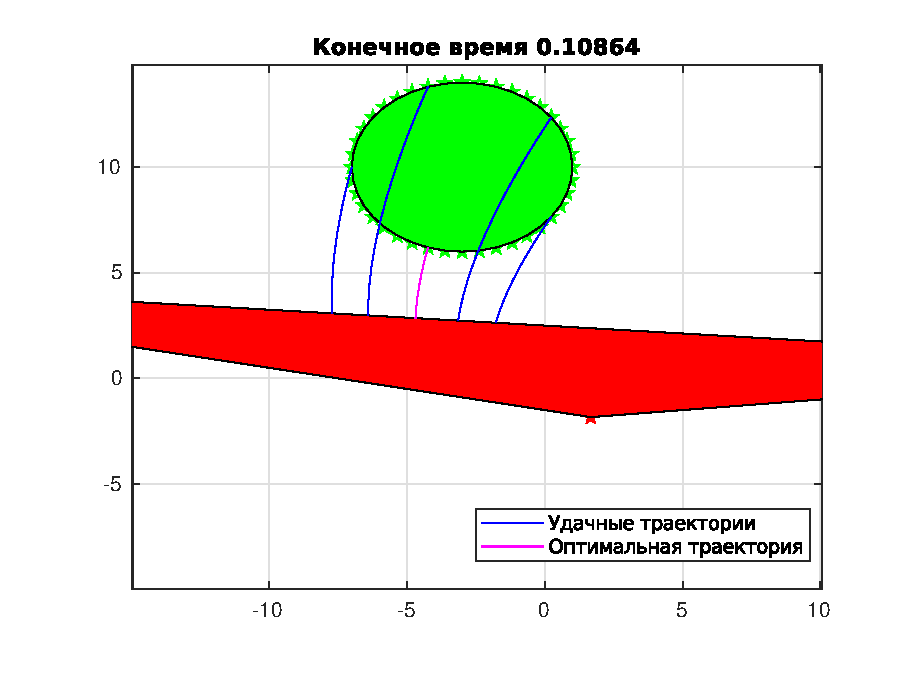
\includegraphics[width=70mm]{algorithm/improvement-1.eps}
                \hfill
                \hfill
                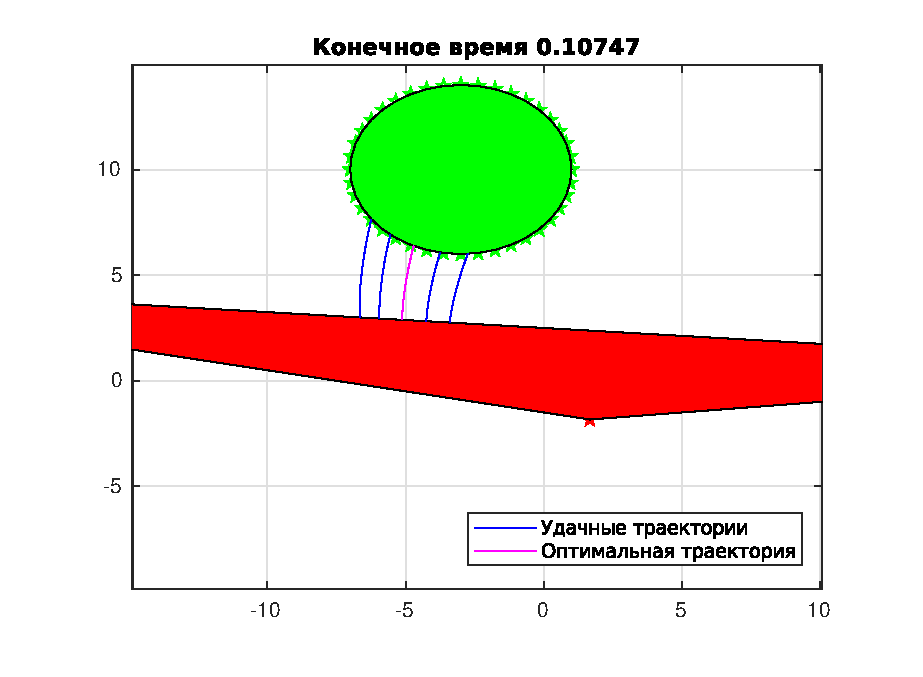
\includegraphics[width=70mm]{algorithm/improvement-2.eps}
                \hfill
                \caption{Пример локального увеличения точности алгоритма.}
        \end{figure}
\end{description}

\begin{remark}
        Очевидно, что в процессе улучшения точности результата работы алгоритма необходимо максимально эффективно использовать полученные на предыдущих итерациях данные. Это значит, что повторное вычисление траекторий системы \eqref{eq:main_system} для уже рассмотренных значений $\psi(t_0)$ производиться не должно.
\end{remark}